N-Gram Graph (NGG) is a NPL tool initially proposed by George Giannakopoulos \cite{Ngram} that uses word or character n-grams in order to achieve documents summarization. The NGG tool basically slices the text in word or character n-grams and then represent them in a graph \emph{G = $\lbrace N,E,L,W\rbrace$} according to the following structure:
% io inserirei prima la definizione di vicino secondo gli NGG
% poi sotto possiamo riutilizzarla. Cosi' mi pare confuso, non si e' mai spiegata la cosa della finestra
\begin{itemize}
	\item N is the set of nodes created for every different n-gram in the text
	\item E represent the edge of the graph; two nodes are connected if they are ``close'' or whithin a \emph{distance window} from each other
	\item L is a labelling function which assigns labels to every node and every edge (define the size of the n-gram)
	\item W is the weight function which assigns weights to every edge according to the number of times that two n-gram appear close one to the other
\end{itemize}

The big advantage coming from the use of this methodology is language
independence, since it makes no assumption on the underlying languages and
allows text manipulation trough graph operations.

In particular two operation are necessary for our goal:
\begin{itemize}
\item the \textbf{Intersection} operator between two graphs $G_1$ and $G_2$: which returns a resulting graph with only the common edges of $G_1$ and $G_2$ averaging the weights of the original edges assigned as the new edge weights(example in figure \ref{fig:IntersectionOperation})
\item the \textbf{Normalized Value Similarity}[NVS] function that for every n-gram rank, indicating how many of the edges contained in graph $G_i$ are also contained in graph $G_j$, considering also the weights of the matching edges and normalize the result respect the graph size
\end{itemize}
 
\begin{figure*}[htbp]
	\centering
			\begin{subfigure}[G1="aaabaab"]
					{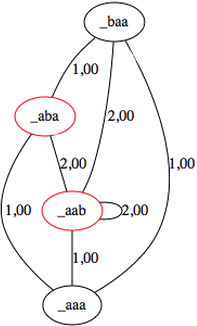
\includegraphics[width=6cm,height=7cm]{image/aaab.png}}	
			\end{subfigure}
			\begin{subfigure}[G2="aabac"]
					{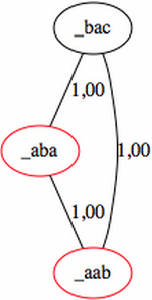
\includegraphics[width=4.5cm,height=7cm]{image/aac.png}}	
			\end{subfigure}
			\begin{subfigure}[Intersection Result]
					{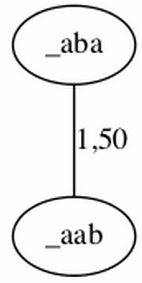
\includegraphics[width=3cm,height=6cm]{image/intersec-res.png}}	
			\end{subfigure}
			\caption[IntersectionOperation]{An example of the intersection operation}
	\label{fig:IntersectionOperation}
\end{figure*}

In particular $NVS(G_i,G_j) = \frac{VS(G_i,G_j)}{SS(G_i,G_j)}$ where:
\begin{equation}
 VS(G_i,G_j)=\frac{\sum e \in G_i \frac{\min(w_e^i, w_e^j)}{\max(w_e^i, w_e^j)}}{\max(\mid G_i \mid, \mid G_j \mid)}
\end{equation}

\begin{equation}
 SS(G_i,G_j)=\frac{\min(\mid G_i \mid, \mid G_j \mid)}{\max(\mid G_i \mid, \mid G_j \mid)}
\end{equation}

Since NGG tools allow to compute both the tweet-news correlation and summary creation, this methodology is split in different section.

\subsubsection*{Tweet-News Correlation}
To compute the correlation between contradiction tweet and news, this methodology use the base idea of exploiting the NVS similarity function as a correlation function: higher the similarity of the tweets n-gram graph representation and the news n-gram representation, higher will be the correlation.

More in detail this procedure perform the following step:
\begin{itemize}
	\item Merge all the tweets corresponding to a CP are in a single document n-gram graph representation.
	\item Compute the news n-gram graph for the news that fall inside a time slots defined by the contradiction point windows increased on both side by a time windows duration
	\item for the news that are inside the time slot, the NVS is computed and represent the correlation value between news and tweet
\end{itemize}

The usage of the time windows is needed given that NVS similarity values have no time domain impact, and with out the time windows isn't possible to  discharge news that are distant in time form the correlation computation.

This approach require a lot of computation, since have to compute the graph representation of all the tweet and for every news inside the time windows compare the tweet with the news text. Instead NGG allow to compute the similarity between text without the usage of grammar information and use this similarity as correlation value: even if has no time relation.


\subsubsection*{Summary Creation}
The second goal of this research is to create a summary of the event that cause the sentiment shift. 

For this purpose we use the news with the highest correlation value obtained at the step before.
Since the goal is to create a summary of 150 word, we suggest to take in consideration only the best 4 news. Increasing the summary length can require more news.

The summary algorithm perform the following action:
\begin{itemize}
	\item sort the news according the correlation value obtained before
	\item save all the sentence of text best $4$ news in a set; the sentence detection is perform using OpenNLP
	\item create the intersection graph of the best $4$ news
	\item for every sentence saved compute the NVS between the sentence n-gram graph and the intersection graph
	\item create the summary using the sentence with the highest NVS value until we reach 150 word
\end{itemize}

this algorithm create a summary composed by the most significant sentence of news with the highest correlation value, but is not able to remove redundant sentence since don't use any semantic index and redundant control. Even this, a summary composed by sentences result to be more human readable than a list of key word.
